La \textit{homepage} del sito ufficiale di Node.js \cite{website:Node.js} fornisce una sintetica ma precisa descrizione di questa tecnologia, un buon punto di partenza per illustrarne le peculiarit�.\\

\begin{figure}[h]
\centering

\includegraphics[width=0.7\linewidth]{./img/nodejs-light}
\caption[Il logo ufficiale di Node.js]{Il logo ufficiale di Node.js}
\label{fig:nodejs-light}
\end{figure}

La descrizione di Node.js riportata sul sito recita:

\begin{quote}
\textit{Node.js is a platform built on Chrome's JavaScript runtime for easily building fast, scalable network applications. Node.js uses an event-driven, non-blocking I/O model that makes it lightweight and efficient, perfect for data-intensive real-time applications that run across distributed devices.}
\end{quote}

E' immediato comprendere che Node.js � una \textit{piattaforma}. L'utilizzo di questo termine mette l'accento su un aspetto fondamentale di questa tecnologia: fornire un ambiente nel quale le applicazioni sviluppate possano funzionare con il supporto di librerie di sistema fornite da Node.js stesso.

La piattaforma Node.js utilizza JavaScript come linguaggio di sviluppo. Per farlo si avvale di una versione appositamente riadattata del potente interprete \textit{V8} presente all'interno del browser \textit{Chrome} di \textit{Google}. L'utilizzo di un linguaggio altamente diffuso e di una base solida come quella fornita dal popolare \textit{browser} permettono di costruire applicazioni affidabili in modo semplice e veloce.

L'ultimo importante concetto, che si apprende dalla prima frase della descrizione, � che Node.js � principalmente orientato allo sviluppo di applicazioni che lavorano con la rete. Per sua natura, la piattaforma ci aiuta a fare in modo che esse siano facilmente scalabili.

La seconda parte della descrizione spiega sinteticamente alcune caratteristiche peculiari di Node.js e ne definisce meglio il contesto applicativo. 

L'intera piattaforma � centrata sul concetto di \textit{evento}. Si dice  evento un messaggio che viene scatenato in un determinato istante dell'elaborazione e che successivamente � catturato e gestito dalle componenti del sistema che sono preposte alla gestione di quell'evento specifico.

Il sistema ad eventi viene utilizzato da Node.js congiuntamente ad una gestione non bloccante delle operazioni di \textit{Input/Output}. Questo significa che una operazione potenzialmente lunga, come ad esempio la comunicazione con il \textit{filesystem} o con i dispositivi di \textit{rete}, non blocca il flusso di esecuzione del programma principale.

Dopo aver richiesto ad altri attori del sistema il dato di cui necessita, il programma continua il suo normale flusso di esecuzione e verr� informato, utilizzando un evento, quando il dato richiesto sar� disponibile. Questa gestione non bloccante delle operazioni di \textit{I/O} � chiamata \textit{I/O asincrono}.

La gestione delle operazioni in modo non strettamente legato alla logica applicativa, permette a Node.js di essere molto efficiente se utilizzato per la realizzazione di applicazioni che manipolano grandi quantit� di dati, ma devono rimanere \textit{reattive} nei confronti di nuove richieste di elaborazione.

\subsection{Le operazioni asincrone}

Interessante, a fronte dell'introduzione del concetto di I/O asincrono, � vedere come Node.js riesca a gestirlo utilizzando una quantit� limitata di risorse di sistema.

I componenti \textit{hardware} di un sistema elaborano dati con velocit� differenti. La rapidit� di ogni componente � fortemente legata al modo nel quale questo � stato realizzato. La tabella seguente riporta un elenco di componenti e le relative velocit� indicative riferite ad un singolo ciclo di \textit{CPU}. 

\begin{center}
\begin{tabular}{l|r}
\textbf{Componente} & \textbf{Numero di cicli} \\ 
\hline 
CPU & 1 \\ 
Cache di livello 1 & 3 \\ 
Cache di livello 2 & 14 \\ 
RAM & 250 \\ 
Hard Disk & 41.000.000 \\ 
Dispositivo di rete & 240.000.000 \\ 
\end{tabular} 
\end{center}

Guardando la tabella si nota immediatamente come i dispositivi di \textit{I/O} siano ordini di grandezza pi� lenti rispetto ai dispositivi di elaborazione delle informazioni. Se il flusso del programma dovesse aspettare, in modo sincrono, ogni singola operazione di lettura o scrittura su disco, ad esempio, esso perderebbe la possibilit� di eseguire circa quaranta milioni di operazioni di calcolo, con un conseguente degrado delle performances del software.

Una tecnica comune per affrontare il problema dell'\textit{I/O} � l'utilizzo di \textit{threads}. Un thread � spesso definito con il termine "sotto-processo leggero", in effetti esso condivide codice e risorse di sistema con altri threads appartenenti allo stesso processo padre.

L'utilizzo dei thread permette ad un processo di parallelizzare l'esecuzione di una parte del suo flusso di lavoro. Al tempo stesso sono necessarie risorse di sistema sia per creare il thread sia per distruggerlo. Node.js ovvia a questo problema utilizzando un \textit{thread pool}, cio� un insieme di thread che fungono da \textit{worker} per il processo. Quando � necessario eseguire un particolare \textit{task}, esso viene sottoposto al thread pool, di conseguenza viene assegnato ad un worker. Esso lo esegue e al termine del lavoro comunica l'esito dell'elaborazione al chiamante tramite una funzione detta \textit{callback}.

L'utilizzo di un thread pool comporta un incremento di prestazioni da parte delle applicazioni che lo sfruttano: i thread pool ottimizzano l'utilizzo della memoria e del processore, diminuendo l'overhead di gestione dei thread.

Per comprendere come Node.js sia in grado di realizzare tale funzionalit�, � necessario spiegare nel dettaglio il modello di gestione delle richieste implementato da questo framework. 

Innanzitutto � necessario chiarire che Node.js, a differenza di altri sistemi per lo sviluppo \textit{server-side} non necessita di una applicazione che funga da \textit{web server}, come accade ad esempio nel caso di Apache per PHP. Quando si sviluppa in Node.js infatti l'applicazione realizzata \textit{�} il server. Il framework mette a disposizione funzionalit� apposite per la creazione di un server interno ad ogni applicazione. Questo approccio favorisce la strutturazione a \textit{servizi} dell'applicazione, che pu� essere suddivisa in processi Node.js separati e quindi in veri e propri server in comunicazione fra loro.

Di seguito � riportato un server web minimale realizzato in Node.js.

\begin{verbatim}
var http = require('http');

http.createServer(function (req, res) {
  res.end('Hello World');
}).listen(3000, '127.0.0.1');

console.log('Server running at http://127.0.0.1:3000/');
\end{verbatim}

La prima operazione eseguita dal programma � l'importazione del modulo \verb|http|, che fornisce le funzionalit� di rete. Successivamente viene chiamata la funzione \verb|createServer()| che si occupa di generare il server web. Utilizzando la funzione \verb|listen()|, successivamente, il server viene attivato e messo in ascolto all'indirizzo \verb|http://127.0.0.1:3000/|. Il comando \verb|console.log()| stampa in console l'informazione che il server � avviato. Ad ogni richiesta ricevuta dal server, viene eseguita la funziona passata come parametro alla \verb|createServer()|, la quale risponde alla richiesta inviando al client la stringa \verb|Hello World|.

Come si vede da questo esempio, con Node.js, la logica applicativa e il \textit{web-server} risiedono all'interno dello stesso software.

Node.js utilizza internamente un modello chiamato \textit{Event Loop} per la gestione delle richieste in arrivo. All'avvio dell'applicazione, vengono attivati un thread principale e un insieme finito (il default � quattro) di thread secondari definiti \textit{thread-pool}. Nell'istante in cui arriva una nuova richiesta da parte di un client, il thread principale la prende in carico ed inserisce i dati della richiesta e la funzione \textit{callback} per gestirla in una coda. A fronte di questa operazione, viene attivato il primo thread libero nel thread-pool, detto \textit{worker}, il quale esegue la callback e raccoglie il risultato. Una volta generato il messaggio di risposta da inviare al client, il worker lo restituisce al thread principale, il quale provvede ad inviarlo al client.

Questo approccio presenta un grande vantaggio rispetto ad altri sistemi non \textit{event-based}: il thread principale � quasi sempre in stato \textit{idle}. Esso si occupa infatti esclusivamente di smistare richieste e raccogliere risposte, quindi rimane sempre reattivo. Il risultato di questo approccio � un sistema responsivo, che riesce a gestire un grande numero di richieste sfruttando una bassissima quantit� di risorse di sistema.

In figura \ref{fig:node-model} � illustrato schematicamente l'event-loop per la gestione delle richieste di Node.js.

\begin{figure}[h]
\centering
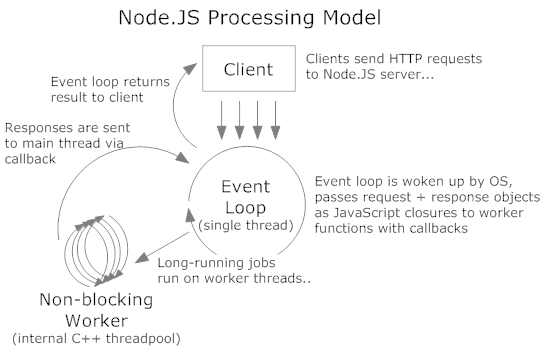
\includegraphics[width=1.0\linewidth]{./img/node-model}
\caption[L'\textit{event loop} di Node.js]{L'\textit{event loop} di Node.js}
\label{fig:node-model}
\end{figure}

\subsection{Le callback}

Una delle principali difficolt� che si presenta ad uno sviluppatore che si appresta ad utilizzare Node.js per la prima volta, � la gestione delle callback. Di seguito � riportato un frammento di codice Node.js che esegue il salvataggio di un utente su Database.

\begin{verbatim}
function save(user) {
  console.log('saving user into db');
  db.insert(user, function(err, user) {
    console.log('user successfully saved!');
  });
  console.log('all we need is just a little patience...');
}
\end{verbatim}

la funzione \verb|db.insert()| � asincrona, ed accetta due parametri: il dato da salvare e la callback da eseguire una volta effettuato l'inserimento nel Database. L'esecuzione di questo codice produce un output in console simile a quello mostrato qui sotto.

\begin{verbatim}
saving user into db
all we need is just a little patience...
user successfully saved!
\end{verbatim}

Se la funzione \verb|db.insert()| non fosse asincrona otterremmo un output come quello che segue.

\begin{verbatim}
saving user into db
user successfully saved!
all we need is just a little patience...
\end{verbatim}

Questo piccolo esempio, lascia intuire un potenziale problema nella gestione delle callback: se, ad esempio, dovessimo assegnare alcuni privilegi di \textit{default} a tutti i nuovi utenti inseriti nel sistema, potremmo scrivere il seguente codice.

\begin{verbatim}
function save(user) {
  console.log('saving user into db');
  db.insert(user, function(err, user) {
  	db.insert(grants, user, function(err, grants) {
      console.log('user successfully saved!');
    });
  });
  console.log('all we need is just a little patience...');
}
\end{verbatim}

Ora il problema � evidente: se i dati ottenuti in modo asincrono sono necessari per eseguire altre procedure, essi vanno gestiti internamente alla callback stessa. Se utilizzate in modo improprio, le callback, portano al cosiddetto \textit{callback-hell}, ovvero un codice nel quale il lettore non riesce pi� a seguire il flusso logico dell'applicazione.

Fortunatamente JavaScript ci fornisce una soluzione semplice al problema, ma che richiede allo sviluppatore disciplina nello scrivere il codice sorgente. L'esempio precedente, infatti potrebbe essere riscritto come segue.

\begin{verbatim}
function onGrantsSaved(err, grants) {
  console.log('user successfully saved!');
}

function onUserSaved(err, user) {
  db.insert(grants, user, onGrantsSaved);
}

function save(user) {
  console.log('saving user into db');
  db.insert(user, onUserSaved);
  console.log('all we need is just a little patience...');
}
\end{verbatim}

Il codice � ora molto pi� leggibile, semplicemente evitando la dichiarazione di funzioni anonime in linea. 

% js nel server
%Questo � un aspetto molto controverso e discusso, infatti se � abituati 
%a pensare tale linguaggio come un "giocattolo", troppo instabile 
%e imprevedibile per 

